\documentclass[11pt,a4paper]{article}

\usepackage[utf8]{inputenc}
\usepackage[T1]{fontenc}
\usepackage{lmodern}
\usepackage[margin=2.2cm,headheight=14pt]{geometry}
\usepackage{xcolor}
\usepackage{graphicx}
\usepackage{amsmath,amssymb}
\usepackage{booktabs}
\usepackage{parskip}
\usepackage{fancyhdr}
\usepackage{tikz}
\usetikzlibrary{arrows.meta,positioning,shapes.geometric,fit,calc}
\usepackage{listings}
\usepackage{hyperref}

\renewcommand{\contentsname}{Table des matières}

% Palette sobre et professionnelle
\definecolor{PrimaryBlue}{HTML}{1E3A5F}
\definecolor{AccentTeal}{HTML}{0F766E}
\definecolor{WarmAmber}{HTML}{B45309}
\definecolor{AlertRed}{HTML}{B91C1C}
\definecolor{SoftBg}{HTML}{F8FAFC}
\definecolor{CodeBg}{HTML}{F1F5F9}
\definecolor{BorderGray}{HTML}{CBD5E1}

\hypersetup{
    colorlinks=true,
    linkcolor=PrimaryBlue,
    urlcolor=AccentTeal,
    pdftitle={Plan d'implémentation 1.0 — HyParView & Plumtree},
    pdfauthor={Ingénierie Systèmes Distribués — Projet Whispernet}
}

% En-têtes et pieds de page
\pagestyle{fancy}
\fancyhf{}
\fancyhead[L]{\small\color{PrimaryBlue}\textbf{Whispernet} — Plan d'implémentation 1.0}
\fancyhead[R]{\small\color{gray}HyParView \& Plumtree}
\fancyfoot[C]{\small\thepage}
\renewcommand{\headrulewidth}{0.4pt}

% Boîtes pédagogiques basées sur TikZ (100% standard)
\newenvironment{pedagogie}[1]{%
    \par\vspace{4pt}\noindent
    \begin{tikzpicture}
        \node[draw=AccentTeal, fill=SoftBg, line width=0.8pt, rounded corners=3pt,
              inner sep=9pt, text width=\dimexpr\linewidth-20pt\relax, align=left] (box) \bgroup
            {\color{AccentTeal}\textbf{#1}}\par\vspace{3pt}
}{%
        \egroup;
    \end{tikzpicture}\par\vspace{4pt}
}

\newenvironment{attention}[1]{%
    \par\vspace{4pt}\noindent
    \begin{tikzpicture}
        \node[draw=WarmAmber, fill=WarmAmber!5, line width=0.8pt, rounded corners=3pt,
              inner sep=9pt, text width=\dimexpr\linewidth-20pt\relax, align=left] (box) \bgroup
            {\color{WarmAmber}\textbf{#1}}\par\vspace{3pt}
}{%
        \egroup;
    \end{tikzpicture}\par\vspace{4pt}
}

% Style du pseudo-code
\lstdefinestyle{pseudocode}{
    backgroundcolor=\color{CodeBg},
    frame=single,
    rulecolor=\color{BorderGray},
    basicstyle=\ttfamily\footnotesize,
    keywordstyle=\color{PrimaryBlue}\bfseries,
    commentstyle=\color{AccentTeal}\itshape,
    stringstyle=\color{WarmAmber},
    numbers=left,
    numberstyle=\tiny\color{gray},
    numbersep=6pt,
    breaklines=true,
    showstringspaces=false,
    tabsize=2,
    inputencoding=utf8,
    extendedchars=true,
    literate=
        {é}{{\'e}}1 {è}{{\`e}}1 {ê}{{\^e}}1 {à}{{\`a}}1 {ù}{{\`u}}1
        {ç}{{\c{c}}}1 {î}{{\^i}}1 {ô}{{\^o}}1 {É}{{\'E}}1 {À}{{\`A}}1
        {œ}{{\oe}}1 {—}{{---}}1 {–}{{--}}1,
    keywords={fn, struct, enum, match, if, else, for, in, return, let, mut, emit, start_timer, cancel_timer, true, false, None, Some}
}
\lstset{style=pseudocode}

\begin{document}

% Page de couverture (cover.png pleine page)
\begin{titlepage}
    \thispagestyle{empty}
    \begin{tikzpicture}[remember picture, overlay]
        \node[inner sep=0pt] at (current page.center) {
            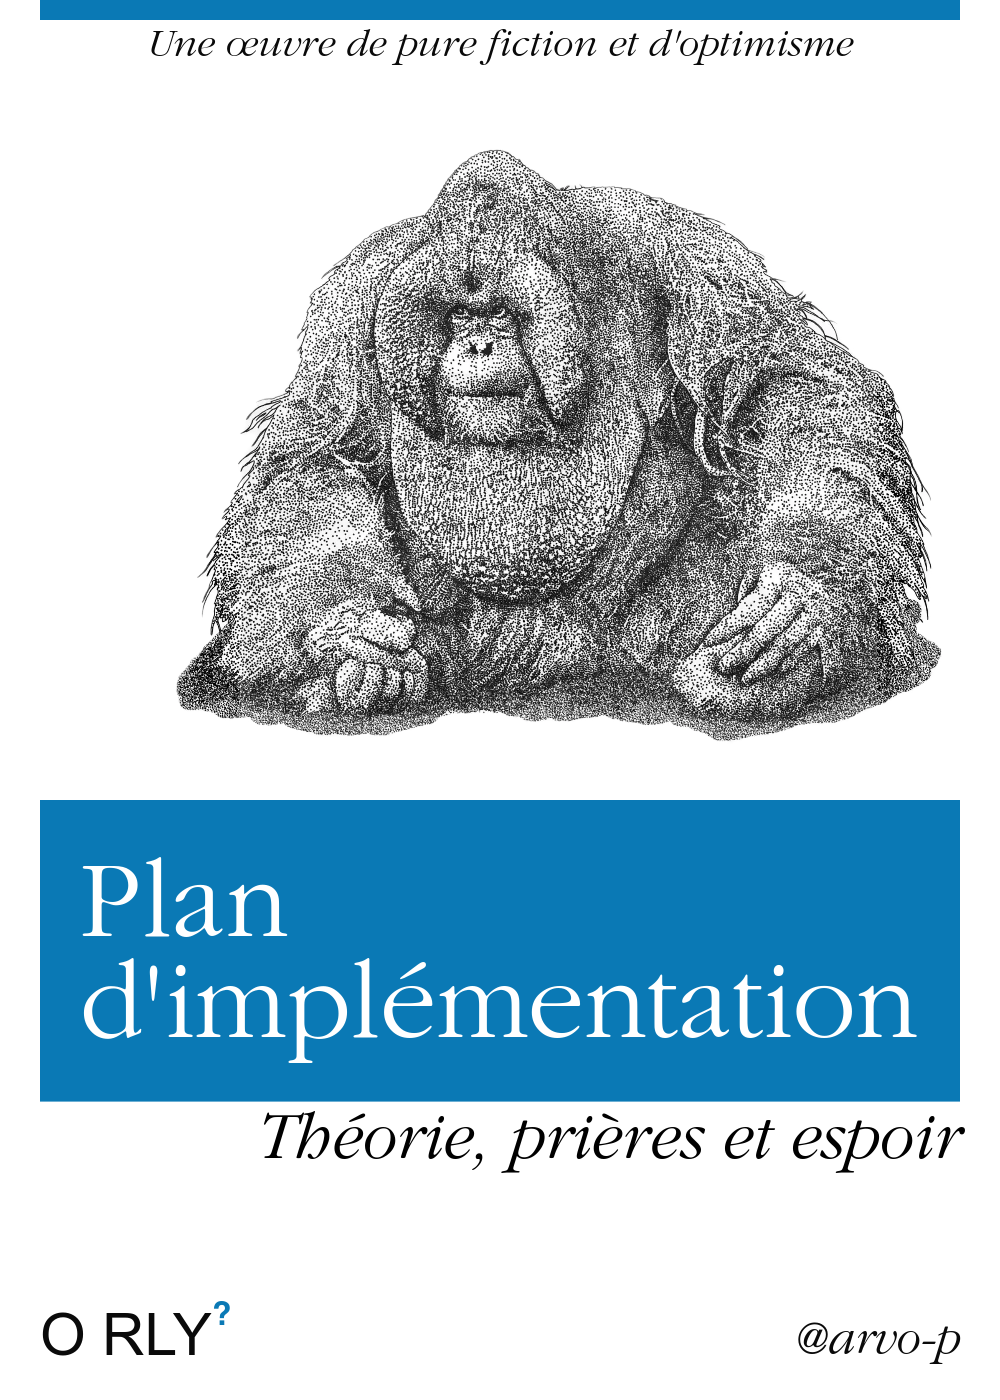
\includegraphics[width=\paperwidth,height=\paperheight]{cover.png}
        };
    \end{tikzpicture}
    \null
\end{titlepage}

\begin{pedagogie}{Objectif du document}
    Ce document constitue le \textbf{Plan d'implémentation 1.0} de la couche de diffusion pair-à-pair de \textbf{Whispernet}. Il sépare clairement les deux protocoles complémentaires — \textbf{HyParView} (gestion de topologie) et \textbf{Plumtree} (diffusion épidémique en arbre) — puis détaille leur couplage selon une architecture \emph{Sans-I/O} déterministe et testable.
\end{pedagogie}

\tableofcontents
\newpage

\section{Introduction}

Bienvenue sur le projet \textbf{Whispernet} ! Whispernet est une application de messagerie de groupe pair-à-pair (P2P) décentralisée et multiplateforme, développée en \textbf{.NET 10} au-dessus de \textbf{N0.IrohNet} (bindings C\# pour la pile réseau QUIC \emph{Iroh}).

L'objectif de ce document est d'offrir à tous les collaborateurs — qu'ils travaillent sur le réseau P2P, l'infrastructure serveur légère ou l'interface graphique — une vision commune et claire de l'architecture du dépôt afin de pouvoir développer en parallèle sans conflits ni duplication de code.

\subsection{Structure du projet et organisation des couches}

La solution \texttt{Whispernet.slnx} est découpée en projets C\# distincts (\emph{1 couche = 1 projet \texttt{.csproj} = 1 namespace racine}), organisés selon une architecture en couches strictement séparées :

\begin{table}[h!]
\centering
\small
\begin{tabular}{@{}llp{6.2cm}@{}}
\toprule
\textbf{Projet / Dossier} & \textbf{Type / Cible} & \textbf{Rôle et responsabilités} \\
\midrule
\texttt{src/Whispernet.Core} & Library (\texttt{net10.0}) & Couche protocole pure \textbf{Sans-I/O} (HyParView + Plumtree). Zéro dépendance réseau ou UI. \\
\texttt{src/Whispernet.Transport.Iroh} & Library (\texttt{net10.0}) & Adaptateur réseau Iroh QUIC (\texttt{N0.IrohNet}). Exécute les \texttt{OutAction} de \texttt{Core} et gère les timers. \\
\texttt{src/Whispernet.App} & Library (\texttt{net10.0}) & Logique applicative partagée et \emph{ViewModels} (salons, historique, commandes), indépendante de l'UI. \\
\texttt{src/Whispernet.Client.Wpf} & WinExe (\texttt{net10.0-windows}) & Interface graphique \textbf{WPF} pour Windows (100\,\% visuelle, liée à \texttt{Whispernet.App}). \\
\texttt{src/Whispernet.Client.Linux} & Exe (\texttt{net10.0}) & Interface utilisateur pour Linux (100\,\% visuelle, liée à \texttt{Whispernet.App}). \\
\texttt{src/Whispernet.MeetingNode} & Exe (\texttt{net10.0}) & Binaire terminal léger 24h/24 pour \textbf{Raspberry Pi / Linux} (utilise \texttt{Core} + \texttt{Transport.Iroh}). \\
\texttt{Tests/} & Exe (\texttt{net10.0}) & Prototype fonctionnel de test de messagerie de groupe P2P (\texttt{demo}, \texttt{host}, \texttt{join}). \\
\texttt{Rapports/} & Documentation & Rapports d'architecture et présent \emph{Plan d'implémentation 1.0}. \\
\bottomrule
\end{tabular}
\caption{Structure complète de la solution \texttt{Whispernet.slnx}}
\end{table}

\begin{pedagogie}{Travailler en parallèle sans se marcher sur les pieds}
Grâce à cette séparation :
\begin{itemize}
    \item Les développeurs \textbf{UI Windows (WPF)} et \textbf{UI Linux} travaillent chacun dans leur projet (\texttt{Client.Wpf} / \texttt{Client.Linux}) en consommant simplement \texttt{Whispernet.App}, sans jamais toucher au code réseau.
    \item Les développeurs \textbf{P2P / Protocole} implémentent HyParView et Plumtree dans \texttt{Whispernet.Core} de manière 100\,\% testable en mémoire.
    \item L'exécutable \textbf{Raspberry Pi (\texttt{MeetingNode})} réutilise directement \texttt{Core} et \texttt{Transport.Iroh} sans embarquer aucune dépendance graphique.
\end{itemize}
\end{pedagogie}

\newpage

\section{Fonctionnalités peer-to-peer}

% ============================================================================
% SECTION 1.1 : HYPARVIEW
% ============================================================================
\subsection{HyParView : Gestion de la topologie et du carnet d'adresses}

Imaginez que vous organisez un grand jeu de piste dans une ville avec 10\,000 participants. Il n'y a pas de chef central, pas de haut-parleur géant, et chacun ne dispose que d'un talkie-walkie à portée limitée. À tout moment, des participants peuvent arriver et d'autres peuvent partir sans prévenir. Comment faire en sorte que personne ne se retrouve jamais isolé, sans obliger tout le monde à appeler 10\,000 personnes ?

C'est le rôle exact de \textbf{HyParView} : \emph{savoir à qui parler} et maintenir un maillage sain, connecté et résistant aux pannes.

\subsubsection{Explication vulgarisée et analogies (Zéro jargon)}

Dans une foule de 10\,000 personnes, personne ne peut serrer la main à tout le monde en même temps. Chacun maintient donc deux listes très différentes, comme dans la vie courante :

\begin{enumerate}
    \item \textbf{La Vue Active (les amis proches au bout du fil)} : c'est un tout petit cercle de personnes (par exemple 4 à 6 personnes) avec lesquelles vous gardez une ligne téléphonique ouverte en permanence. Vous savez à la seconde près si l'une d'elles raccroche ou tombe en panne. C'est à travers ces quelques personnes que vous parlez au reste du monde.
    \item \textbf{La Vue Passive (le répertoire de secours)} : c'est une liste plus grande (par exemple 20 à 30 noms) de personnes que vous avez croisées ou dont on vous a parlé, mais que vous n'appelez pas pour l'instant. Si l'un de vos amis proches (Vue Active) disparaît brutalement, vous piochez immédiatement un remplaçant dans ce répertoire de secours pour ne jamais rester isolé.
\end{enumerate}

\begin{pedagogie}{Le mécanisme de \emph{Shuffle} : échanger des cartes de visite}
Si vous ne mettez jamais votre répertoire à jour, il finira par contenir des numéros périmés de personnes rentrées chez elles. Pour éviter cela, chaque participant fait régulièrement un \textbf{Shuffle} (un brassage) : il prend quelques noms dans son carnet, les met dans une enveloppe, et l'envoie à travers la foule. Le destinataire ouvre l'enveloppe, ajoute ces nouveaux contacts dans son propre répertoire, et renvoie en échange quelques noms tirés du sien. Résultat : même sans serveur central, tout le monde garde un répertoire frais, varié et représentatif du groupe actuel.
\end{pedagogie}

\subsubsection{Fonctionnement concret pas-à-pas (Scénario A, B, C, D, E, F)}

Considérons un réseau composé initialement de 5 nœuds : \textbf{A, B, C, D, E}, avec une capacité maximale de Vue Active fixée à 3 voisins par nœud pour simplifier la lecture.
\textbf{État initial} : A connaît \{B, C, D\} dans sa Vue Active ; B connaît \{A, C, E\} ; C connaît \{A, B, D\} ; D connaît \{A, C, E\} ; E connaît \{B, D\}.

\subsubsection*{Scénario 1 : Arrivée d'un nouveau nœud F (\texttt{JOIN})}
Le nouveau nœud \textbf{F} démarre et ne connaît qu'un seul point d'entrée (nœud de contact) : \textbf{A}.
\begin{enumerate}
    \item \textbf{F} envoie un message \texttt{JOIN} à \textbf{A}.
    \item \textbf{A} accepte \textbf{F} dans sa Vue Active. Comme sa Vue Active était pleine (\{B, C, D\}), A libère une place : il choisit un voisin au hasard (disons \textbf{D}), ferme la connexion active avec D via \texttt{DISCONNECT} et déplace D dans sa \emph{Vue Passive} (D fait de même pour A).
    \item \textbf{A} crée ensuite un message \texttt{FORWARD\_JOIN(F, ttl = ARWL)} (avec un nombre de sauts max \texttt{ARWL}, par ex. 4) et l'envoie à tous ses autres voisins actifs (\textbf{B} et \textbf{C}).
    \item \textbf{B} et \textbf{C} reçoivent \texttt{FORWARD\_JOIN(F)}, décrémentent le \texttt{ttl} et le relaient aléatoirement vers \textbf{E} et \textbf{D}.
    \item Quand le \texttt{ttl} atteint une valeur intermédiaire (\texttt{PRWL}, ex. 2 sauts), le nœud qui le reçoit (disons \textbf{E}) ajoute \textbf{F} dans sa \emph{Vue Passive} pour diversifier les répertoires.
    \item Lorsque le \texttt{ttl} atteint \textbf{0} (chez \textbf{D} et \textbf{E} selon les chemins), ces nœuds établissent une connexion active directe avec \textbf{F} via \texttt{NEIGHBOR(high\_priority = true)}.
\end{enumerate}
\textbf{Résultat} : \textbf{F} est intégré au maillage avec plusieurs voisins actifs répartis dans le réseau (\textbf{A}, \textbf{D}, \textbf{E}).

\subsubsection*{Scénario 2 : Panne brutale du nœud B et remplacement}
Supposons que \textbf{B} tombe brutalement en panne (coupure réseau ou crash) :
\begin{enumerate}
    \item La couche transport signale à \textbf{A} et à \textbf{E} que la connexion vers \textbf{B} est perdue (\texttt{on\_connection\_lost(B)}).
    \item \textbf{E} retire immédiatement \textbf{B} de sa Vue Active.
    \item Pour combler le trou dans sa Vue Active, \textbf{E} pioche un candidat aléatoire dans sa \emph{Vue Passive} (disons \textbf{C}) et lui envoie \texttt{NEIGHBOR(high\_priority = true)} (priorité haute si sa Vue Active est vide, normale sinon).
    \item \textbf{C} accepte et ajoute \textbf{E} à sa Vue Active (et réciproquement). HyParView a restauré la connectivité du maillage.
\end{enumerate}

\subsubsection{Architecture d'implémentation Sans-I/O (HyParView)}

\subsubsection*{Structures de données et messages réseau}

\begin{lstlisting}[caption={État en mémoire et messages réseau propres à HyParView}]
struct HyParViewState {
    self_id: NodeId,
    active_view: Set<NodeId>,          // Capacité max k_active (ex: 5)
    passive_view: Set<NodeId>,         // Capacité max k_passive (ex: 30)
    pending_neighbors: Set<NodeId>,    // Connexions en cours d'établissement
}

enum HyParViewMessage {
    Join { sender: NodeId },
    ForwardJoin { new_node: NodeId, ttl: u8, sender: NodeId },
    Neighbor { sender: NodeId, high_priority: bool },
    NeighborAck { sender: NodeId, accepted: bool },
    Disconnect { sender: NodeId },
    Shuffle { origin: NodeId, sample: Vec<NodeId>, ttl: u8 },
    ShuffleReply { sample: Vec<NodeId> },
}
\end{lstlisting}

\subsubsection*{Pseudo-code des fonctions principales (\texttt{on\_connection\_lost}, \texttt{shuffle})}

\begin{lstlisting}[caption={Gestion de perte de connexion et brassage périodique dans HyParView}]
fn on_connection_lost(state: &mut NodeState, dead_peer: NodeId) {
    if state.hyparview.active_view.remove(dead_peer) {
        // Notifier la couche supérieure (Plumtree)
        on_neighbor_down(state, dead_peer);

        // Remplacer le pair perdu depuis la Vue Passive
        let high_prio = state.hyparview.active_view.is_empty();
        if let Some(candidate) = pop_random(&mut state.hyparview.passive_view) {
            state.hyparview.pending_neighbors.insert(candidate);
            emit(OutAction::Connect(candidate));
            emit(OutAction::Send(candidate, NetworkMessage::HyParView(
                HyParViewMessage::Neighbor {
                    sender: state.hyparview.self_id,
                    high_priority: high_prio,
                }
            )));
        }
    }
}

fn shuffle(state: &mut NodeState) {
    if state.hyparview.active_view.is_empty() {
        return;
    }
    let target = pick_random(&state.hyparview.active_view);
    let mut sample = Vec::new();
    sample.push(state.hyparview.self_id);
    sample.extend(pick_random_subset(&state.hyparview.active_view, K_ACTIVE_SAMPLE));
    sample.extend(pick_random_subset(&state.hyparview.passive_view, K_PASSIVE_SAMPLE));

    emit(OutAction::Send(target, NetworkMessage::HyParView(
        HyParViewMessage::Shuffle {
            origin: state.hyparview.self_id,
            sample,
            ttl: SHUFFLE_ARWL,
        }
    )));
}
\end{lstlisting}

\newpage

% ============================================================================
% SECTION 2 : PLUMTREE
% ============================================================================
\subsection{Plumtree : Diffusion épidémique en arbre et auto-réparation}

Maintenant que HyParView garantit à chaque nœud un petit cercle de 4 à 6 amis proches fiables, comment diffuser une nouvelle à travers les 10\,000 participants sans que tout le monde la reçoive en quadruple ? C'est le rôle exact de \textbf{Plumtree} (\emph{Push-Lazy-Push Multicast Tree}).

\subsubsection{Explication vulgarisée et analogies (Zéro jargon)}

Si vous envoyez chaque nouvelle à tous vos 5 amis, qui l'envoient chacun à leurs 5 amis, les chemins forment des boucles : les mêmes messages tournent en rond et gaspillent la bande passante. \textbf{Plumtree} résout ce problème en classant vos amis proches (ceux de votre Vue Active) en deux catégories :

\begin{itemize}
    \item \textbf{Les pairs \emph{Eager} (les destinataires directs)} : ce sont les amis à qui vous envoyez le message \textbf{en entier} dès que vous le recevez. Ils forment les branches d'un arbre de diffusion rapide : chaque personne ne reçoit théoriquement le message qu'une seule fois, par le chemin le plus court.
    \item \textbf{Les pairs \emph{Lazy} (le filet de sécurité)} : ce sont vos autres amis proches. Au lieu de leur envoyer tout le message (ce qui ferait doublon), vous leur envoyez juste un petit SMS discret : \emph{« Hé, au fait, j'ai reçu l'info n°42 »}. Cela ne coûte presque rien, mais ça leur permet de vérifier qu'ils ne l'ont pas ratée.
\end{itemize}

Comment ce tri se fait-il automatiquement ? Grâce à deux réflexes simples :
\begin{itemize}
    \item \textbf{\emph{Prune} (élaguer une branche en trop)} : si vous recevez le message n°42 en entier de la part de Bob, alors qu'Alice vous l'a déjà envoyé une fraction de seconde plus tôt, vous dites gentiment à Bob : \emph{« Merci Bob, mais je l'ai déjà eu par ailleurs. À partir de maintenant, ne m'envoie plus les messages complets, préviens-moi juste par petit SMS (passe en mode Lazy). »} Le réseau coupe ainsi automatiquement les chemins redondants.
    \item \textbf{\emph{Graft} (greffer une branche de secours)} : si votre ami Alice tombe en panne, vous ne recevez plus le message n°43. Mais Bob (qui était en mode \emph{Lazy}) vous envoie son petit SMS : \emph{« J'ai l'info n°43 »}. Vous attendez un tout petit instant au cas où l'info arriverait par un autre chemin. Si rien ne vient, vous répondez à Bob : \emph{« J'ai raté le n°43 ! Envoie-le-moi tout de suite, et désormais envoie-moi tous les messages en entier (passe en mode Eager). »} L'arbre vient de se réparer tout seul.
\end{itemize}

\subsubsection{Fonctionnement concret pas-à-pas (Scénario A, B, C, D, E)}

\subsubsection*{Scénario 1 : Envoi d'un message normal et élagage d'un doublon (\texttt{PRUNE})}
Supposons que l'arbre démarre (tous les liens actifs sont initialement \emph{Eager}). \textbf{A} publie le message \texttt{M1} (\emph{« Réunion à 14h »}).

\begin{center}
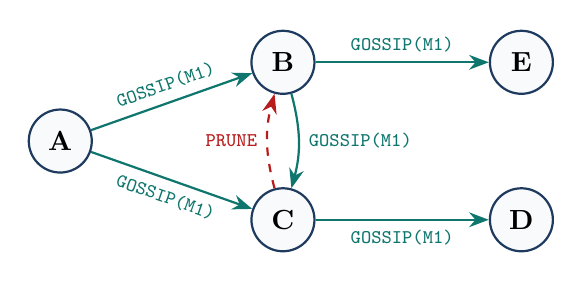
\begin{tikzpicture}[
    node distance=1.6cm,
    peer/.style={circle, draw=PrimaryBlue, thick, fill=SoftBg, minimum size=8mm, font=\bfseries},
    eager/.style={-{Stealth[length=2.5mm]}, thick, AccentTeal},
    prune/.style={-{Stealth[length=2.5mm]}, thick, dashed, AlertRed}
]
    \node[peer] (A) {A};
    \node[peer, right=2cm of A, yshift=1cm] (B) {B};
    \node[peer, right=2cm of A, yshift=-1cm] (C) {C};
    \node[peer, right=2.2cm of B] (E) {E};
    \node[peer, right=2.2cm of C] (D) {D};

    \draw[eager] (A) -- node[above, sloped, font=\scriptsize] {\texttt{GOSSIP(M1)}} (B);
    \draw[eager] (A) -- node[below, sloped, font=\scriptsize] {\texttt{GOSSIP(M1)}} (C);
    \draw[eager] (B) -- node[above, font=\scriptsize] {\texttt{GOSSIP(M1)}} (E);
    \draw[eager] (C) -- node[below, font=\scriptsize] {\texttt{GOSSIP(M1)}} (D);
    \draw[eager, bend left=15] (B) to node[right, font=\scriptsize] {\texttt{GOSSIP(M1)}} (C);
    \draw[prune, bend left=15] (C) to node[left, font=\scriptsize, color=AlertRed] {\texttt{PRUNE}} (B);
\end{tikzpicture}
\end{center}

\begin{enumerate}
    \item \textbf{A} enregistre \texttt{M1} dans son historique des messages vus, puis envoie \texttt{GOSSIP(M1, round=0)} à ses pairs \emph{Eager} (\textbf{B} et \textbf{C}).
    \item \textbf{B} reçoit \texttt{GOSSIP(M1)} de A pour la première fois : il le livre à l'application, l'enregistre, et le relaie à ses pairs \emph{Eager} (\textbf{C} et \textbf{E}) avec \texttt{round=1}.
    \item Entre-temps, \textbf{C} avait \emph{déjà} reçu \texttt{M1} directement de A (en 1 seul saut). Quand \textbf{C} reçoit le doublon \texttt{GOSSIP(M1)} envoyé par B :
    \begin{itemize}
        \item \textbf{C} ignore le contenu (déjà livré).
        \item \textbf{C} déplace \textbf{B} de son ensemble \emph{Eager} vers son ensemble \emph{Lazy}.
        \item \textbf{C} envoie un message \texttt{PRUNE} à \textbf{B}.
    \end{itemize}
    \item Quand \textbf{B} reçoit \texttt{PRUNE} de C, \textbf{B} déplace également \textbf{C} de son ensemble \emph{Eager} vers son ensemble \emph{Lazy}.
\end{enumerate}
\textbf{Résultat} : Le lien B $\leftrightarrow$ C est élagué pour les gros messages. Au prochain message \texttt{M2}, B n'enverra plus le corps de \texttt{M2} à C, mais seulement un court identifiant \texttt{IHAVE(id=M2)}.

\subsubsection*{Scénario 2 : Réparation de l'arbre après la panne de B (\texttt{IHAVE} et \texttt{GRAFT})}
Reprenons la suite de la panne de \textbf{B} vue dans HyParView : \textbf{A} vient de publier \texttt{M2}, mais \textbf{B} tombe en panne avant de le relayer à \textbf{E}.
\begin{enumerate}
    \item \textbf{D} a bien reçu \texttt{M2} via le chemin A $\rightarrow$ C $\rightarrow$ D. Or \textbf{D} a \textbf{E} dans son ensemble \emph{Lazy} (lien élagué précédemment).
    \item À la fin de son timer périodique \emph{Lazy}, \textbf{D} envoie un résumé \texttt{IHAVE(id=M2, round=2)} à \textbf{E}.
    \item \textbf{E} reçoit \texttt{IHAVE(M2)} et consulte son historique : \emph{« Je n'ai jamais vu M2 ! »}.
    \item \textbf{E} enregistre cette annonce et démarre un court timer de grâce (\texttt{IHaveTimer}, ex. 100 ms) au cas où \texttt{M2} serait déjà en route par une autre branche.
    \item Le timer expire sans que \texttt{M2} soit arrivé : \textbf{E} déclenche la réparation :
    \begin{itemize}
        \item \textbf{E} déplace \textbf{D} de \emph{Lazy} vers \emph{Eager}.
        \item \textbf{E} envoie \texttt{GRAFT(id=M2)} à \textbf{D}.
    \end{itemize}
    \item \textbf{D} reçoit \texttt{GRAFT(M2)} : il déplace \textbf{E} de \emph{Lazy} vers \emph{Eager}, retrouve \texttt{M2} dans son cache local de messages récents, et le renvoie immédiatement à \textbf{E} via \texttt{GOSSIP(M2)}.
\end{enumerate}
\textbf{Résultat} : \textbf{E} reçoit le message manquant \texttt{M2} et le lien D $\rightarrow$ E devient une branche \emph{Eager} permanente pour tous les messages suivants.

\subsubsection{Architecture d'implémentation Sans-I/O (Plumtree)}

\subsubsection*{Structures de données et messages réseau}

\begin{lstlisting}[caption={État en mémoire et messages réseau propres à Plumtree}]
struct PlumtreeState {
    eager_peers: Set<NodeId>,          // Sous-ensemble de active_view
    lazy_peers: Set<NodeId>,           // Complément dans active_view
    received_msgs: Map<MsgId, Payload>,// Historique borné (LRU / TTL) pour dédup et GRAFT
    missing_ihaves: Map<MsgId, Queue<(NodeId, Round)>>, // Annonces en attente de timer
    lazy_queue: Vec<(NodeId, MsgId, Round)>,            // IHAVE en attente d'envoi groupé
}

enum PlumtreeMessage {
    Gossip { msg_id: MsgId, round: u32, payload: Bytes },
    Prune,
    IHave { entries: Vec<(MsgId, u32)> }, // (msg_id, round)
    Graft { msg_id: MsgId, round: u32 },
}
\end{lstlisting}

\subsubsection*{Pseudo-code des fonctions principales (\texttt{on\_receive\_gossip}, \texttt{on\_receive\_ihave})}

\begin{lstlisting}[caption={Traitement de réception d'un Gossip et d'un IHave dans Plumtree}]
fn on_receive_gossip(state: &mut NodeState, from: NodeId, msg_id: MsgId, round: u32, payload: Bytes) {
    if !state.plumtree.received_msgs.contains_key(msg_id) {
        // Premier contact avec ce message : livraison et diffusion
        state.plumtree.received_msgs.insert(msg_id, payload.clone());
        emit(OutAction::DeliverToApp(msg_id, payload.clone()));

        // Annuler une éventuelle réparation en cours pour ce message
        if state.plumtree.missing_ihaves.remove(msg_id).is_some() {
            emit(OutAction::CancelTimer(TimerKind::IHaveTimer(msg_id)));
        }

        // Si le message vient d'un pair Lazy, on le promeut en Eager
        if state.plumtree.lazy_peers.remove(from) {
            state.plumtree.eager_peers.insert(from);
        }

        // Diffusion Eager + mise en file Lazy
        for peer in state.plumtree.eager_peers {
            if peer != from {
                emit(OutAction::Send(peer, NetworkMessage::Plumtree(
                    PlumtreeMessage::Gossip { msg_id, round: round + 1, payload: payload.clone() }
                )));
            }
        }
        for peer in state.plumtree.lazy_peers {
            if peer != from {
                state.plumtree.lazy_queue.push((peer, msg_id, round + 1));
            }
        }
    } else {
        // Doublon : on élague la branche redondante
        if state.plumtree.eager_peers.remove(from) {
            state.plumtree.lazy_peers.insert(from);
        }
        emit(OutAction::Send(from, NetworkMessage::Plumtree(PlumtreeMessage::Prune)));
    }
}

fn on_receive_ihave(state: &mut NodeState, from: NodeId, entries: Vec<(MsgId, u32)>) {
    for (msg_id, round) in entries {
        if state.plumtree.received_msgs.contains_key(msg_id) {
            continue;
        }
        let first_annonce = !state.plumtree.missing_ihaves.contains_key(msg_id);
        state.plumtree.missing_ihaves.entry(msg_id).or_default().push_back((from, round));
        if first_annonce {
            emit(OutAction::StartTimer(TimerKind::IHaveTimer(msg_id), IHAVE_TIMEOUT));
        }
    }
}
\end{lstlisting}

\begin{pedagogie}{Complément sur \texttt{on\_ihave\_timeout(msg\_id)}}
Lorsque \texttt{IHaveTimer(msg\_id)} expire et que \texttt{msg\_id} n'est toujours pas dans \texttt{received\_msgs}, la machine à états retire le premier couple \texttt{(peer, round)} de \texttt{missing\_ihaves[msg\_id]}, promeut \texttt{peer} en \texttt{eager\_peers}, émet \texttt{Send(peer, Graft \{ msg\_id, round \})}, et relance le timer au cas où \texttt{peer} ne répondrait pas (permettant ainsi d'essayer le prochain pair de la file).
\end{pedagogie}

\newpage

% ============================================================================
% SECTION 3 : SYNERGIE ET COUPLAGE SANS-I/O
% ============================================================================
\subsection{Synergie et couplage complet (HyParView + Plumtree)}

\subsubsection{Pourquoi forment-ils un duo complémentaire ?}

\begin{center}
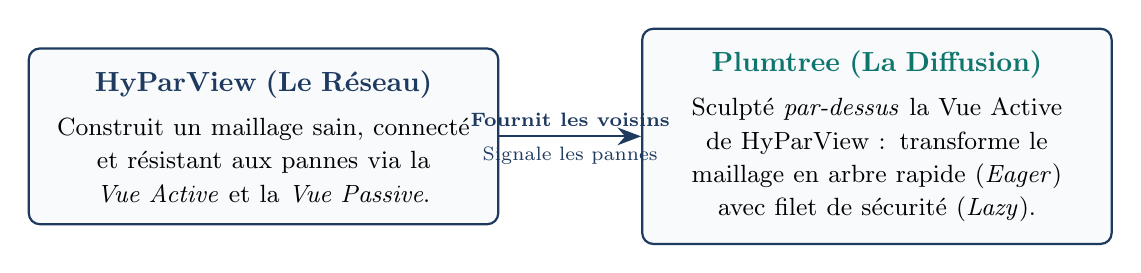
\begin{tikzpicture}[
    node distance=1.4cm,
    box/.style={draw=PrimaryBlue, thick, rounded corners=4pt, fill=SoftBg, text width=5.4cm, align=center, inner sep=8pt}
]
    \node[box] (hypar) {\textbf{\color{PrimaryBlue}HyParView (Le Réseau)}\\[4pt]\small Construit un maillage sain, connecté et résistant aux pannes via la \emph{Vue Active} et la \emph{Vue Passive}.};
    \node[box, right=1.8cm of hypar] (plum) {\textbf{\color{AccentTeal}Plumtree (La Diffusion)}\\[4pt]\small Sculpté \emph{par-dessus} la Vue Active de HyParView : transforme le maillage en arbre rapide (\emph{Eager}) avec filet de sécurité (\emph{Lazy}).};
    \draw[-{Stealth[length=3mm]}, thick, PrimaryBlue] (hypar.east) -- node[above, font=\scriptsize\bfseries] {Fournit les voisins} node[below, font=\scriptsize] {Signale les pannes} (plum.west);
\end{tikzpicture}
\end{center}

HyParView sans Plumtree permet de rester connecté, mais chaque diffusion sature le réseau de doublons. Plumtree sans HyParView ne sait pas qui contacter au départ ni comment trouver de nouveaux voisins quand plusieurs amis disparaissent. Ensemble :
\begin{enumerate}
    \item \textbf{HyParView} s'occupe de la \emph{santé des connexions} : il garantit que chaque nœud garde quelques voisins fiables et remplace les morts instantanément.
    \item \textbf{Plumtree} s'occupe de \emph{l'efficacité de la parole} : il réutilise exactement ces voisins pour bâtir un arbre sans doublon, tout en utilisant les liens élagués (\emph{Lazy}) comme bouée de sauvetage en cas de panne.
\end{enumerate}

\subsubsection{Architecture globale Sans-I/O et couplage}

L'approche \textbf{Sans-I/O} (\emph{State Machine Pattern}) sépare strictement la logique pure du réseau (QUIC/Iroh, sockets, timers OS) : la machine à états reçoit des événements et retourne une liste d'actions (\texttt{OutAction}) à exécuter.

\begin{lstlisting}[caption={État global unifié, messages et actions de sortie Sans-I/O}]
struct NodeState {
    hyparview: HyParViewState,
    plumtree: PlumtreeState,
}

enum NetworkMessage {
    HyParView(HyParViewMessage),
    Plumtree(PlumtreeMessage),
}

enum OutAction {
    Connect(NodeId),
    CloseConnection(NodeId),
    Send(NodeId, NetworkMessage),
    DeliverToApp(MsgId, Bytes),
    StartTimer(TimerKind, Duration),
    CancelTimer(TimerKind),
}
\end{lstlisting}

\begin{attention}{Invariant critique de cohérence}
À tout moment, l'union des ensembles Plumtree doit correspondre exactement à la Vue Active de HyParView :
\[
\texttt{eager\_peers} \cup \texttt{lazy\_peers} = \texttt{active\_view}
\qquad \text{et} \qquad
\texttt{eager\_peers} \cap \texttt{lazy\_peers} = \emptyset
\]
Toute mutation de \texttt{active\_view} (ajout ou suppression) doit immédiatement déclencher \texttt{on\_neighbor\_up(peer)} (ajout à \texttt{eager\_peers}) ou \texttt{on\_neighbor\_down(peer)} (retrait de \texttt{eager\_peers} et \texttt{lazy\_peers}).
\end{attention}

\subsubsection{Timers et événements déclencheurs indispensables}

\begin{table}[h!]
\centering
\small
\begin{tabular}{@{}lllp{5.8cm}@{}}
\toprule
\textbf{Timer / Événement} & \textbf{Protocole} & \textbf{Fréquence / Délai} & \textbf{Rôle exact} \\
\midrule
\texttt{ShuffleTimer} & HyParView & Périodique (ex. 10--30 s) & Envoie un \texttt{Shuffle} pour rafraîchir \texttt{passive\_view}. \\
\texttt{LazyPushTimer} & Plumtree & Périodique (ex. 50--100 ms) & Regroupe et envoie les \texttt{IHAVE} de \texttt{lazy\_queue}. \\
\texttt{IHaveTimer(msg\_id)} & Plumtree & Ponctuel (ex. 100--300 ms) & Attend avant d'envoyer \texttt{GRAFT} si le message tarde. \\
\texttt{NeighborUp(peer)} & Couplage & Sur ajout à \texttt{active\_view} & Ajoute \texttt{peer} dans \texttt{eager\_peers}. \\
\texttt{NeighborDown(peer)} & Couplage & Sur perte de connexion & Retire \texttt{peer} de \texttt{eager\_peers} et \texttt{lazy\_peers}. \\
\bottomrule
\end{tabular}
\caption{Timers et événements internes nécessaires à l'orchestration Sans-I/O}
\end{table}

\subsection{Idées}
\subsubsection{Raspberry PI : Point de Meeting 24/24}

Dans un réseau pair-à-pair pur, un problème classique apparaît lorsqu'un utilisateur démarre son application alors que ses anciens contacts sont hors ligne : il ne sait plus à qui envoyer son premier \texttt{JOIN}. Déployer un ou plusieurs \textbf{Raspberry Pi} allumés 24h/24 comme \emph{Points de Meeting} (nœuds d'amorçage et de rendez-vous) résout ce problème tout en conservant une architecture décentralisée.

\paragraph{1. Rôle du Point de Meeting dans le réseau P2P.}
Le Raspberry Pi n'est pas un serveur central qui relaie toutes les conversations : c'est un nœud spécialisé du maillage qui assure la découvrabilité :
\begin{itemize}
    \item \textbf{Identité stable et disponibilité continue} : tout comme un client qui persiste sa clé pour garder son identité utilisateur, le Raspberry Pi sauvegarde sa \texttt{SecretKey} Iroh sur disque (ex. \texttt{/var/lib/whispernet/identity.key}) afin de conserver un \texttt{EndpointId} fixe. La différence clé est que les clients ont une \emph{présence réseau intermittente} (PC éteint, veille, changement de Wi-Fi), alors que le Point de Meeting reste joignable 24h/24 et peut donc être embarqué comme point d'ancrage fiable dans la configuration par défaut.
    \item \textbf{Stockage et redistribution des \texttt{EndpointId}} : le Point de Meeting exécute \textbf{HyParView} avec une \emph{Vue Passive} élargie (ex. 100 à 500 entrées au lieu de 30). Dès qu'un client rejoint le réseau (\texttt{JOIN}) ou effectue un \texttt{Shuffle}, le Raspberry Pi enregistre son \texttt{EndpointId} (ainsi que ses adresses/relais) et lui redistribue un échantillon de pairs actifs récemment vus.
    \item \textbf{Identification explicite (\texttt{NodeRole::MeetingPoint})} : lors des échanges HyParView (\texttt{Join}, \texttt{Neighbor}, \texttt{Shuffle}), chaque nœud annonce son rôle (\texttt{Peer} standard ou \texttt{MeetingPoint}). Cette distinction permet :
    \begin{itemize}
        \item aux clients de conserver les \texttt{MeetingPoint} comme \emph{ancre de secours} prioritaire si leur \texttt{active\_view} et leur \texttt{passive\_view} deviennent vides ;
        \item au Point de Meeting de fonctionner optionnellement en mode \textbf{HyParView-only} (ou de refuser le rôle \emph{Eager} dans Plumtree) afin de ne pas saturer sa bande passante et sa carte SD avec le trafic applicatif, tout en assurant la topologie.
    \end{itemize}
\end{itemize}

\paragraph{2. Architecture en couches pour un déploiement léger sur Linux.}
Pour que le même cœur protocolaire tourne aussi bien sur un poste client (Windows/Linux avec interface) que en programme de terminal ultra-léger sur Raspberry Pi (\texttt{linux-arm64}), le projet doit être découpé en couches strictement indépendantes :

\begin{center}
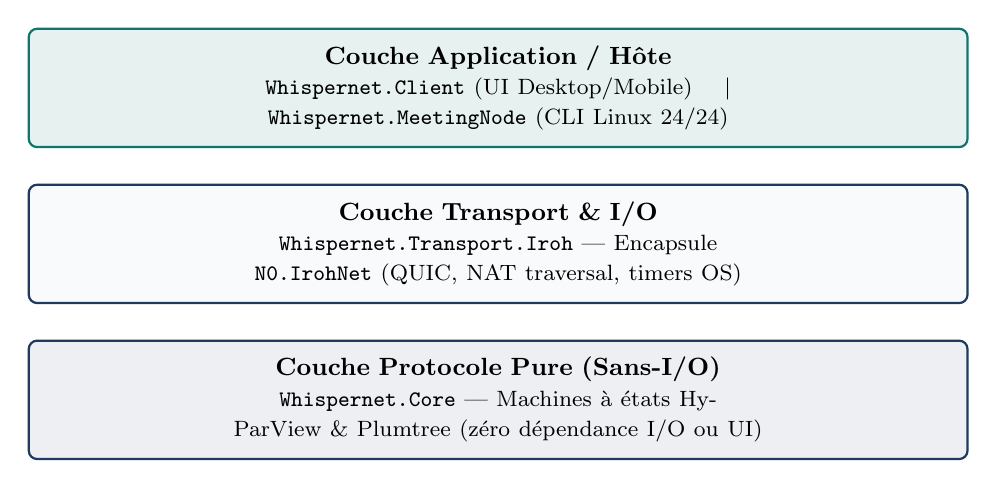
\begin{tikzpicture}[
    node distance=0.45cm,
    layer/.style={draw=PrimaryBlue, thick, rounded corners=3pt, fill=SoftBg, text width=11.5cm, align=center, inner sep=6pt, font=\small}
]
    \node[layer, fill=AccentTeal!10, draw=AccentTeal] (ui) {\textbf{Couche Application / Hôte} \\ \footnotesize \texttt{Whispernet.Client} (UI Desktop/Mobile) \quad $\vert$ \quad \texttt{Whispernet.MeetingNode} (CLI Linux 24/24)};
    \node[layer, below=of ui] (transport) {\textbf{Couche Transport \& I/O} \\ \footnotesize \texttt{Whispernet.Transport.Iroh} — Encapsule \texttt{N0.IrohNet} (QUIC, NAT traversal, timers OS)};
    \node[layer, below=of transport, fill=PrimaryBlue!8] (core) {\textbf{Couche Protocole Pure (Sans-I/O)} \\ \footnotesize \texttt{Whispernet.Core} — Machines à états HyParView \& Plumtree (zéro dépendance I/O ou UI)};
\end{tikzpicture}
\end{center}

\begin{itemize}
    \item \textbf{\texttt{Whispernet.Core}} : contient uniquement les structures \texttt{HyParViewState}, \texttt{PlumtreeState} et la logique pure. Compilable partout sans aucune dépendance native.
    \item \textbf{\texttt{Whispernet.Transport.Iroh}} : exécute les \texttt{OutAction} via \texttt{N0.IrohNet} (qui fournit nativement les binaires \texttt{linux-arm64} pour Raspberry Pi via \texttt{N0.IrohNet.NativeAssets.Linux}).
    \item \textbf{\texttt{Whispernet.MeetingNode}} : un simple exécutable console sans interface graphique (\texttt{OutputType=Exe}), piloté par CLI ou fichier de configuration, très peu gourmand en RAM et facilement supervisé par \texttt{systemd} (\texttt{Restart=always}) sur Raspberry Pi OS / Arch Linux ARM.
\end{itemize}

\end{document}
